% ---------------------------------------------------
%
% Trabajo de Fin de Grado. 
% Author: Laura Padrón Jorge. 
% Capítulo: La aplicacion BulletPoint. 
% Fichero: Cap4_TheApplication.tex
%
% ----------------------------------------------------
%

\chapter{La aplicación BulletPoint} \label{chap:LaAplicacion} 

En este capítulo trataremos diversos temas relacionados con la aplicación, comenzaremos por definir posibles casos de uso en el ámbito universitario, tocaremos diversos temas relacionados incluyendo dificultades durante el desarrollo y acabaremos discutiendo posibles líneas futuras de desarrollo.

 
\section{Aplicaciones móviles en entornos universitarios}


Actualmente las posibilidades de las aplicaciones móviles para entornos universitarios se presentan amplias, cada universidad intenta tener su propia aplicación siguiendo un patrón similar. Realizando una investigación general de las aplicaciones disponibles en el mercado observamos que estas aplicaciones se centran en ofrecer servicios propios (servicio de correo, moodle, chat entre usuarios,etc), mantener al alumno informado y agilizarle los trámites mayoritariamente. 

En un principio, estas aplicaciones se enfocaban a atraer alumnos, centrandose en la calidad de la universidad y mostrando las posibilidades que ofrecían, sin embargo, con el paso de los años y el desarrollo creciente de las aplicaciones móviles, se muestra un cambio en esta estrategia. Ahora las aplicaciones tienen una doble función, no sólo buscan el acceso de nuevos estudiantes sino que también intentan mejorar la experiencia de los alumnos existentes y acercar a los nuevos a la experiencia de la universidad. 


Algunos ejemplos posibles los encontramos en el marketplace de google:

\begin{itemize}
\item Universidad Galileo: \cite{URL::galileo}
\item Univerisidad de Valladolid: \cite{URL::valladolid}
\item Universidad de Oviedo: \cite{URL::oviedo}
\end{itemize}


Uno de los hechos que podemos observar es que las universidades están intentando obtener una solución rápida para desarrollar su app, una de estas soluciones es la creación de plantillas web optimizadas de su sitio web, lo que podemos considerar una opción rápida con un coste bajo.


Hoy en día casi todos los estudiantes tienen acceso a un dispositivo móvil y cuentan con una tarifa de internet. En un futuro próximo con la aparición de estos dispositivos ya nos surge la pregunta ¿Serán capaces estos dispositivos de transformar la educación? y en caso aformativo ¿De que manera? 

\section {Posibles casos de uso de la tecnología beacon en entornos universitarios}

Como mencionaba antes, una de las posibilidades que se presentan para explotar esta tecnología se encuentra en las instituciones de enseñanza, las cuales podrían utilizar los beacons para facilitar a sus alumnos, profesores y demás personal involucrado  una serie de servicios de gran utilidad.


Sin embargo, para utilizar esta tecnología es necesario cumplir una serie de condiciones:

\begin{itemize}
\item Tener instalada la aplicación en su dispositivo móvil.
\item Tener activado el bluetooth.
\item La aplicación ha de estar "despierta".
\item Los beacons han de estar desplegados y configurados correctamente en lugares clave donde el rango sea óptimo.
\end{itemize}

En el caso de dispositivos Apple no es necesario tener activado el bluetooth ya que el SO se encarga de captar las señales BLE, aparte tampoco es necesario que la app esté despierta ya que nuevamente el SO se encarga de despertar a la aplicación involucrada. Sin embargo Apple no ha desarrollado un IBeacon físico aún, aunque en un futuro, se espera que sus dispositivos móviles puedan funcionar como un beacon bidirecional. Cabe destacar que existen librerías que se encargan de realizar estas mismas funcionalidades para mantener el móvil despierto a la escucha de posibles beacon para otros Sistemas Operativos, pero a diferencia de Apple esta funcionalidad no está integrada directamente en el Sistema Operativo por lo que no presenta el mismo nivel de control.


Asimismo, podemos afirmar que prácticamente la mayoría de las universidades cuentan con una disposición amplia en lo que se refiere a servicios y despliegue de medios. Como ejemplo, podemos coger la Universidad de la Laguna, la cual cuenta con una red WiFi con un rango de cobertura casi completo de sus instalaciones y una amplia carta de servicios disponibles para sus alumnos. Además cuenta con una serie de Beacons, que podrían ser instalados fácilmente en lugares estratégicos. 

Partiendo de esta base, procederemos a explorar posibles casos de uso para los beacons tomando el contexto universitario y del alumnado como referente:

\subsection{Guía a través del Campus de la Universidad}

Este caso de uso cubre la funcionalidad destacada de un beacon, el posicionamiento y guía tanto en exteriores como en interiores. 

Como interesados podríamos destacar: 

\begin{itemize}
\item Personal invitado a jornadas o eventos en instalaciones de la Universidad.
\item Alumnos de intercambio en programas internacionales.
\item Alumnos de nuevo acceso.
\item Personas con discapacidad.
\end{itemize}

\begin{figure}[h]
	\centering
	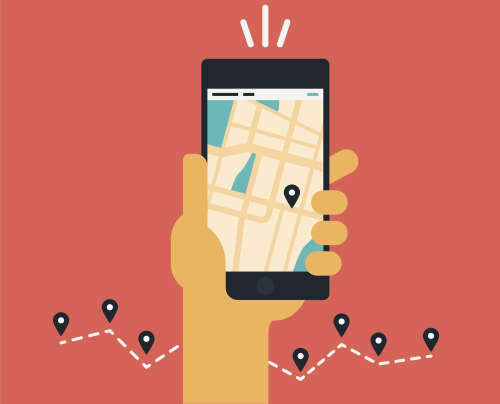
\includegraphics[width=\columnwidth]{locationMobileBeacon}
	\caption{Servicios de localización a través de la Universidad}
	\label{fig:beaconLocation}
\end{figure}

El funcionamiento sería el siguiente: 

El usuario transita por las inmediaciones del campus universitario. El usuario accede al sistema de navegación dentro de la aplicación. La aplicación le muestra entonces el camino mostrándole en todo momento su ubicación como un punto de color sobre el mapa del campus. Este mapa tiene marcados puntos de interés que contienen información de diferente tipo dependiendo del punto marcado: nombre, historia, página web, teléfono de contacto, trámites asociados... son algunos de los datos que podría mostrar. El mapa se va actualizando dependiendo de la posición del usuario permitiendo volver a la vista más alejada en cualquier momento para una visualización más general.


\subsection{Descarga automática de material}

Este caso de uso resultaría muy útil para personal lectivo y para estudiantes, los cuales accederían de manera más sencilla al material dado. También sería aplicable para ponentes de charlas los cuales no tendrían que colgar sus apuntes en alguna plataforma externa o llevarlos consigo en  un almacenamiento externo para compartirlo al finalizar.

El funcionamiento sería el siguiente: 

El profesor o ponente lleva consigo un beacon y sus estudiantes u oyentes tienen instalados en sus dispositivos la aplicación. El profesor es capaz de introducir en su aplicación con el perfil de profesor (el poniente con su correspondiente perfil), indicaciones del material a utilizar en el evento. El profesor carga consigo el pequeño dispositivo e indica a sus alumnos que conecten el bluetooth y abran la aplicación, al entrar en el rango, la aplicación pedirá permiso al alumno para descargarse el contenido indicado por el profesor. Si el alumno acepta, la aplicación pasaría a abrir  el contenido indicado por la página correspondiente.


\subsection{Acceso al parking y conteo de número de vehículos estacionados}


Este caso de uso proporcionaría información muy útil a los usuarios del parking de la universidad, informando del número coches estacionados en el parking y de las plazas restantes a ocupar en tiempo real.

El funcionamiento sería el siguiente: 

El personal de la Ull tendría la aplicación en su móvil, al acercarse a la barrera del parking, el usuario activaría el bluetooth de su móvil. El beacon por su parte registraría un nuevo punto entrando en el rango de acción del parking. La aplicación comprobaría que el usuario está autorizado a entrar en el parking y procedería a abrir la puerta del parking dejando entrar al vehículo. Cuando el vehículo saliese del rango del beacon por el rango interior, la aplicación registraría entonces un nuevo acceso al parking y contabilizaría otro vehículo dentro de parking. Al salir del parking el proceso sería el mismo, por lo tanto la aplicación sería capaz de informar al usuario de las plazas ocupadas en tiempo real.


\subsection{Gestión de eventos e información, entrada automática}

El funcionamiento sería el siguiente: 

Los alumnos transitan los interiores de la Universidad de camino a sus clases. Los beacons están desplegados en las inmediaciones de lugares de interés, tipo aularium, paraninfo, clases que se utilicen a modo de salas de reuniones o seminarios. Al pasar por las inmediaciones de estos lugares de interés, la aplicación sería capaz de proporcionar al usuario información de diversa índole: ponientes, tema de la charla, acceso, teléfono de contacto u otra información similar.  Al mismo tiempo, la aplicación también cuenta con un tablón donde se muestran posibles eventos futuros. Estos eventos pueden ser muy variados y corresponder a diferentes tipos de actividades. Al mismo tiempo se podría confirmar la entrada al evento en el caso de haberla, mediante un código de acceso identificativo generado al realizar el pago del evento.

\begin{figure}[H]
	\centering
	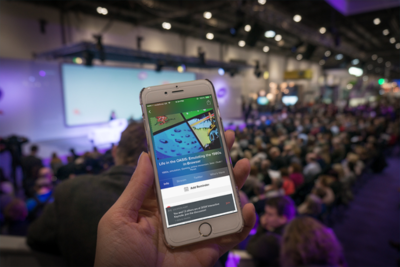
\includegraphics[width=\columnwidth]{BeaconEvent}
	\label{fig:eventBeacon}
\end{figure}

\subsection{Despacho del profesorado e información}

El funcionamiento podría abarcarse de dos maneras, por un lado, podría utilizarse para proveer a los alumnos de información acerca del grupo de despachos, aclarando que profesores tienen el despacho en la zona, horario de tutorías, correo electrónico de contacto, horario de corrección de exámenes, etc. De esta manera el alumno al acercarse a la zona sería capaz de saber información de todos los profesores, o si buscase a alguno en particular, la aplicación le daría la opción de elegir su nombre de una lista y simplemente comprobar si tiene su despacho en esa zona. 

Por otro lado, este caso de uso podría abarcarse para proporcionar una información adicional, comprobando si el profesor está en la zona en ese momento y se encuentra disponible. El profesor tendrá un perfil de la aplicación con un código identificativo que le distingue de los demás profesores. Estos datos se guardarían en un servicio externo, y el beacon sería el encargado de registrar las entradas y salidas de los profesores. En cuanto al estado de disponibilidad, sería un dato que actualizaría el profesor desde su perfil de profesor en la aplicación. Los alumnos recibirían estos estados desde su lado de la aplicación y serían capaces de saber cuando el profesor se encuentra disponible mediante la aplicación. 

\subsection{Información y descuentos para usuarios de la APP}

Este caso de uso no solo dependería de la universidad, sino de establecimientos comerciales interesados. La idea sería la siguiente: 

La universidad en colaboración con un establecimiento comercial le entrega un beacon. La aplicación contaría con un perfil para el dueño del establecimiento, donde sería capaz de introducir información que quiere que se muestre al usuario al pasar cerca de su establecimiento, mensajes de información, descuentos u ofertas especiales por ejemplo. El usuario al pasar por las inmediaciones del establecimeinto recibe en su aplicación una notificación del establecimiento con la información introducida por el dueño anteriormente. Al aceptar la notificación, el usuario podría ser redirigido a la página web del establecimiento para ver la mejor oferta \textcolor[rgb]{0,1,0}{o simplemente descartarla????}. En cualquier caso el establecimiento ha conseguido captar la atención de un posible cliente, y el usuario se benefiaría de ofertas y descuentos. 

\subsection{Control de asistencia}

Este caso de uso podría ir ligado al de Descarga automática de material, el funcionamiento sería el siguiente: 

El alumno conectaría el bluetooth de su móvil al iniciar la clase, en este momento la aplicación detectaría los dispositivos con los identificadores de alu de los alumnos y los dejaría registrados a la clase en el horario establecido. Los profesores serían capaces en todo momento desde su perfil de profesor de consultar asistencia. Si lo unimos con la descarga automática de material que ya habíamos mencionado en apartados anteriores, proporcionaría comodidad tanto a alumnos como a profesores. Sin embargo, un impedimento podría ser el rango del beacon o la necesidad de activar el bluetooth ya que, si el alumno no tiene batería en el móvil, tendría que haber un método secundario. 

\subsection{Control de acceso a instalaciones}

En control de acceso a las aulas y edificios puede ser un tema abordable mediante el uso de estos dispositivos, los lectores de tarjetas pasarían a ser algo innecesario. El alumno simplemente tendría que activar el bluetooth cerca del punto de acceso, se comprobaría su identificador y procedería a darle a acceso o a informarle de su falta de permiso para acceder. El acceso a estos puntos podría quedar guardado en algún tipo de plataforma donde se monitorizen los accesos dependiendo de la seguridad de acceso al aula.

\subsection{Biblioteca Informativa}

Otro posible uso que se le podría dar a esta tecnología tiene que ver con las bibliotecas o lugares de almacenamiento de material. El alumno se acercaría a la biblioteca buscando un libro específico, en la aplicación estaría registrado la localización de los libros disponibles en los estantes, lo que le indicaría al alumno la posición del libro que busca. Para lugares amplios donde hay gran cantidad de material, incluso podría guiar al usuario como un punto por las instalaciones hasta llegar a su objetivo, informarle de si quedan ejemplares disponibles o de fecha prevista de entrada de algún material, de esta manera el alumno agilizaría su búsqueda en gran medida.

\begin{figure}[H]
	\centering
	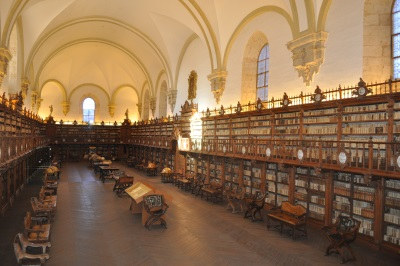
\includegraphics[width=\columnwidth]{BibliotecaSalamanca}
	\caption{La biblioteca de la Universidad de Salamanca (USAL) contiene más de 1.000.000 de ejemplares lo que puede hacer dificil la localización de algunos títulos.}
	\label{fig:bibliotecaUSAL}
\end{figure}

\subsection{Actividades interactivas por el Campus, jornadas de acogida u otros eventos}

En un aspecto más recreativo, se podría tener en cuenta el uso de los beacons para organizar juegos o actividades divertidas para los alumnos. Estos eventos dependerían de los organizadores, pero podrían consistir en alguna actividad que implicase movimiento y colaboración. Los alumnos tendrían que registrarse con su identificador, una ruta a través del campus con adivinanzas o puzzles que tengan que ver con diferentes temáticas por ejemplo fomentaría a los alumnos a trabajar en equipo y utilizar su ingenio.Al mismo tiempo se podría aplicar algún tipo de recompensa para los ganadores, descuentos o bonos tramitados por medio de la aplicación, lo que fomentaría la participación estudiantil.

\subsection{Localización de transporte público, horarios e información de la parada}

Teniendo en cuenta los medios de transporte que utilizan los estudiantes, uno de los principales es el autobus. Este medio de transporte puede llegar a ser el día a día de muchos de los estudiantes que no cuentan con vehículo propio o que simplemente prefieren utilizar el autobus. 

Este caso de uso contempla lo siguiente: 


El estudiante llega a una parada de autobus y utilizando su dispositivo móvil, consulta los autobuses que van a pasar por la parada; la aplicación le permite obtener información de los diferentes autobuses, el itinerario y los minutos que faltan para que llege a la parada, asimismo también enlazaría con la web de la compañía de transporte para más información sobre las líneas y los itinerarios en caso de necesitar más información que la proporcionada por la aplicación.

\section{Casos de uso elegidos}

Como ya hemos mencionado previamente, estos casos de uso se incluyen como parte de una aplicación mayor, donde cada caso de uso se considera un módulo. La integración de cada uno de estos módulos con el resto de la aplicación se ha enlazado mediante el desarrollo de un menú de funcionalidades donde es posible seleccionar qué acción deseamos realizar. Para contener los datos necesarios para algunos módulos, se ha introducido un menú adicional de ajustes. Estos datos se utilizan entre otras cosas para identificar al alumno y confirmar ciertas acciones o dejar constancia de otras. A continuación se desglosarán los distintos casos de uso en los que tendremos que pensar de ahora en adelante como módulos.

\subsection{Localización de transporte público, horarios e información de la parada}

\subsubsection{Objetivo}


El objetivo de este caso de uso es el conocer, en tiempo real, qué autobuses pasan por la parada en la que nos encontramos, hacia donde se dirigen, y cuánto tiempo falta para que llegen a la parada. En caso de necesidad de información adicional, la aplicación está preparada para enviarnos a navegar por la página web de la empresa (TITSA) , donde podemos ver más datos sobre el autobús seleccionado.


\subsubsection{Despliegue}

En este caso, sería necesario colocar un beacon en cada parada de guaguas. De esta manera cada parada de guagua queda identificada por un beacon. Si el usuario se encuentra cercano a dos paradas, la aplicación considera que le interesa la información de la parada más cercana a su posición y le proporcionará información únicamente de esta parada con el objetivo de no confundir al usuario.


\subsubsection{Funcionamiento}


Mediante el uso de los beacons, permitimos a la aplicación identificar en que parada se encuentra el usuario. La aplicación asocia la MAC de un beacon con el número identificativo de la parada. Este número identificativo de la parada es lo que utiliza TITSA para identificar sus paradas en la API y en toda su web.

\begin{figure}[H]
	\centering
	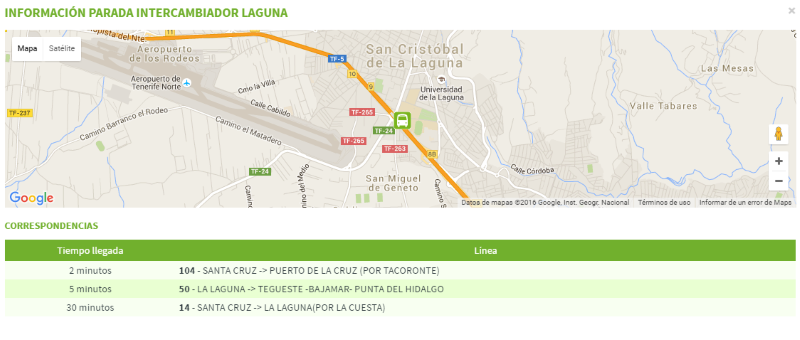
\includegraphics[width=\columnwidth]{titsaMap}
	\caption{Actualmente la información mostrada por titsa en su página web.}
	\label{fig:MapaTitsa}
\end{figure}

La aplicación ha sido programada enlazando los números identificativos de la parada con la dirección MAC de los beacons. Cuando la aplicación detecta un beacon es capaz de reconocer la parada en la que se encuentra el usuario. Una vez la aplicación conoce los datos de la parada, se procede a realizar dos peticiones de comunicación con el servicio de TITSA: 

\begin{itemize}
\item La primera petición se hace sobre la API de TITSA que nos proporciona la información de los autobuses y el tiempo que queda para que llege dicho autobús a la parada. Cabe destacar que para poder utilizar esta API nos pusimos en contacto con TITSA, la cual nos proporcionó una API KEY para poder trabajar con ella.
\item La segunda petición se realiza sobre la página de TITSA directamente. El objetivo de esta petición es obtener de cada guagua la información del recorrido del autobús. Se obtiene el código de la página en html y para cada autobus se extrae la información relativa a su itinerario, la información no se encuentra en un formato óptimo en muchos casos, pero es un vistazo rápido al itinerario.
\end{itemize}


A parte de esta información por cada autobus se incluye un link a modo de botón, que redireciona al usuario a la página web de TITSA con el identificador de la línea, con lo que el usuario puede obtener más información en caso de duda.

En un principio, la idea era utilizar simplemente la API de TITSA, puesto que se creía que proporcionaría toda esta información, sin embargo en algunos casos, los destinos no se correspondían, y las rutas salían erróneas. Ante esta situación, nos pusimos en contacto con alguien que estaba involucrado en esta API quien nos comentó que esto ocurría en algunos casos por la manera en la que estaba planteada la API.


La solución a la que se llegó, fue utilizar ambos métodos para obtener la información completa. Ambos métodos serán desglosados a continuación: 


En el primer método, utilizando una librería de peticiónes HTTP, se manda una consulta por GET a la API de TITSA que nos devuelve una respuesta en XML, esta respuesta se parsea con un Handler de XML. Al mismo tiempo, se inicia la petición a la página de TITSA y utilizando JSOUP, se obtiene el contenido de la página web. De este contenido en html, recopilamos únicamente el recorrido de los autobuses y el resto se descarta. Esta petición es bastante más pesada que la del xml previa, ya que tiene que obtener todo el contenido de la página web en la que aparece el desglose del itinerario en formato html. El parseo de la página también es más lento que en el paso previo, ya que tiene que ir elemento por elemento iterando en los elementos hijos del html.


Utilizando ambos conjuntos de datos, se va creando una estructura con los datos, donde se almacena la información sobre cada elemento. En última instancia se van añadiendo estos elementos a la vista utilizando un adaptador y una estructura para visualizar listas.

\begin{figure}[H]
	\centering
	\includegraphics[width=120mm,height=170mm]{autobuses}
	\caption{Podemos conocer en tiempo real, autobuses que se acercan a la parada, junto con su destino y tiempo de llegada de la parada identificada por un beacon.}
	\label{fig:autobuses}
\end{figure}


\subsubsection{Dificultades}


A la hora de plantear este caso de uso se han tenido dificultades: 

\begin{itemize}
\item A la hora de presentar los datos, la generación de la estructura era un proceso con el que no se estaba familiarizado y que ha llevado más tiempo del previsto, pero que ha servido de piedra angular para el desarrollo de los demás casos de uso ya que presenta elementos comunes: peticiones, parseo de datos, visualización de listas, etc.
\item Otra dificultad ha sido el no poder obtener todos los datos necesarios con una sola petición y tener que hacer uso de dos peticiones distintas, con el tratamiento posterior de estos datos, ya que no eran en absoluto similares.
\end{itemize}

Estos han sido las principales dificultades, sin embargo el trato por parte de TITSA siempre ha sido favorable, participando y respondiendo las consultas rápidamente y facilitando el desarrollo.


\subsubsection{Ampliación}

Ampliar este caso de uso sólo conllevaría asociar los nuevos identificadores de los beacons a nuevos identificadores de parada. Por ello podemos afirmar que sería relativamente sencillo desplegar una red de beacons en las paradas de guagua de TITSA en este caso y obtener esta información de manera sencilla. 


\subsection{Gestión de eventos e información}

\subsubsection{Objetivo}

El objetivo de este caso de uso sigue siendo el de proporcionar información de eventos e información de interés para el usuario; sin embargo, se han desligado de la parte de la entrada automática, al que hacíamos mención en el análisis previo, ya que en la mayoría de los casos no es necesaria esta funcionalidad.  


\subsubsection{Despliegue}


En este caso, sería necesario colocar un beacon en sitios de interés donde puedan tener lugar eventos. Al mismo tiempo, también es necesaria una fuente de datos donde poner la información de los eventos. De esta manera cada beacon referenciaría a una fuente de información de eventos. Si el usuario se encuentra cercano a dos beacons, la aplicación considera que le interesa la información del beacon más cercano a su posición, si se desplaza a otra posición y se acerca a otro beacon, la información sería diferente.

\subsubsection{Funcionamiento}


Mediante el uso de los beacons, permitimos a la aplicación identificar en que localización se encuentra el usuario. En este caso, hemos utilizado la información RSS de la página web eventosUll (referencia). Esta página posee diferentes enlaces RSS, actualmente no están separados por ubicación sino por categorías variadas (ocio, eventos, deportes, tecnologías,etc) sin embargo lo hemos tomado de ejemplo porque es algo que ya está en funcionamiento y que proporciona información sobre eventos actuales relacionados con la Universidad de la Laguna. 


\begin{figure}[H]
	\centering
	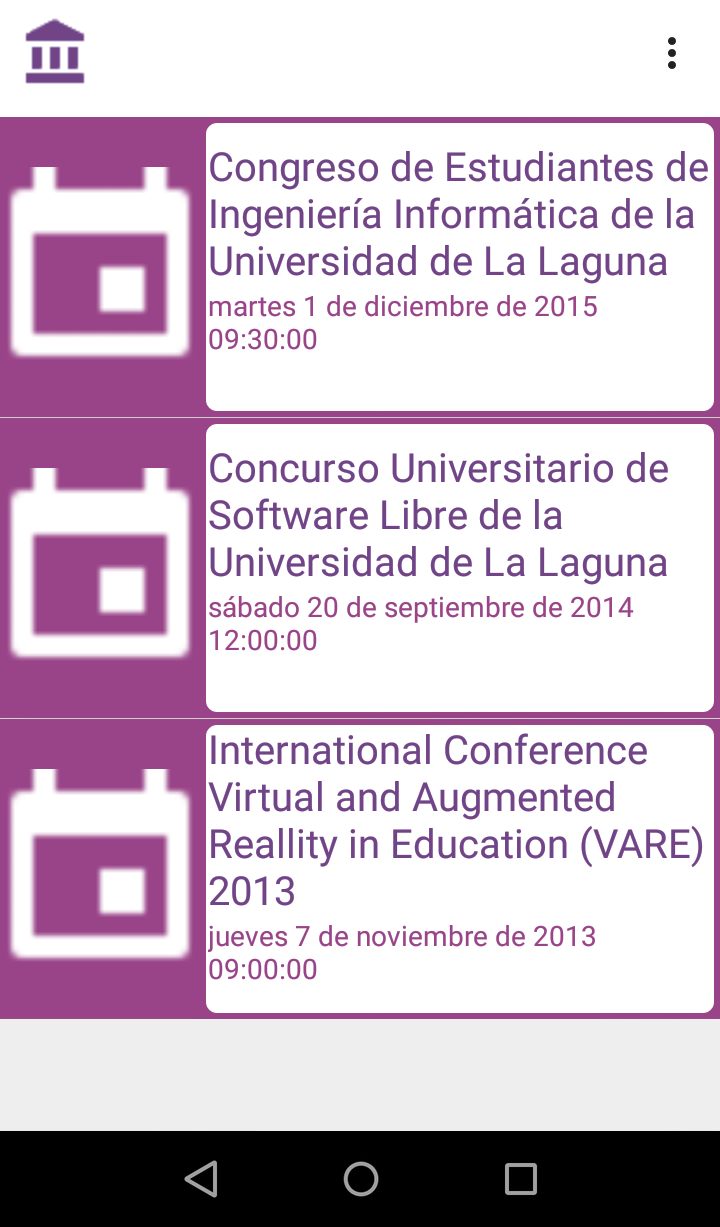
\includegraphics[width=120mm,height=170mm]{Eventos}
	\caption{Podemos conocer eventos asociados a un RSS de la página web de eventos.ull.}
	\label{fig:eventos}
\end{figure}

La aplicación ha sido programada enlazando la dirección MAC de los beacons con diferentes links RSS de la página web de eventos. Al detectar un beacon, se reconoce a qué información queremos acceder y se procede a realizar una petición utilizando el link identificado por el beacon: 


La petición se lanza sobre el link el cual nos devuelve un archivo XML que procedemos a tratar para sacar la información que nos interesa. Para no sobrecargar la aplicación con demasiada información del evento hemos decidido utilizar sólo los datos más relevantes. En principio, el título y la fecha del evento. Al mismo tiempo, sobre cada evento se incluye un link que al seleccionar nos envía a la página web del evento seleccionado para darnos más información sobre él (localización en un mapa, manera de inscribirse al evento, etc) sin embargo, esta información no la contienen todos los eventos.


En un principio, se planteó el filtrar los eventos para obtener los cercanos a una posición geográfica; sin embargo, no todos los eventos poseen esta información, y sería necesario realizar una petición por cada RSS para obtener los datos con lo que se tardaría mucho más y el proceso sería más lento. Si en el futuro se planteara, cada RSS debería estar en función de la localización del evento.

\begin{figure}[H]
	\centering
	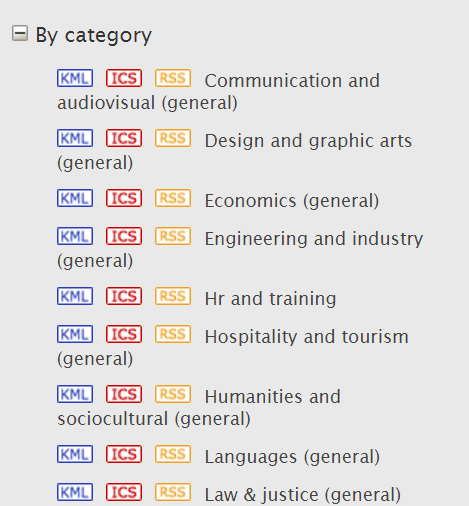
\includegraphics[width=\columnwidth]{eventsRss}
	\caption{Las diferentes categorías de los RSS de la página web de eventos.ull.es}
	\label{fig:eventsRss}
\end{figure}


La petición se realiza utilizando la misma librería de peticiónes HTTP que en el caso anterior: se envía una consulta por GET al link RSS de la página web de eventosULL que nos devuelve una respuesta en XML. Esta respuesta se parsea con un Handler de XML para seleccionar únicamente los datos que nos interesan. Esta petición es bastante rápida y genera una vista con la información de los distintos eventos. Cada elemento evento de esta lista es capaz de enviarnos a la página web de eventosULL para recibir más información en caso de estar interesados en el evento en cuestión.

\begin{figure}[H]
	\centering
	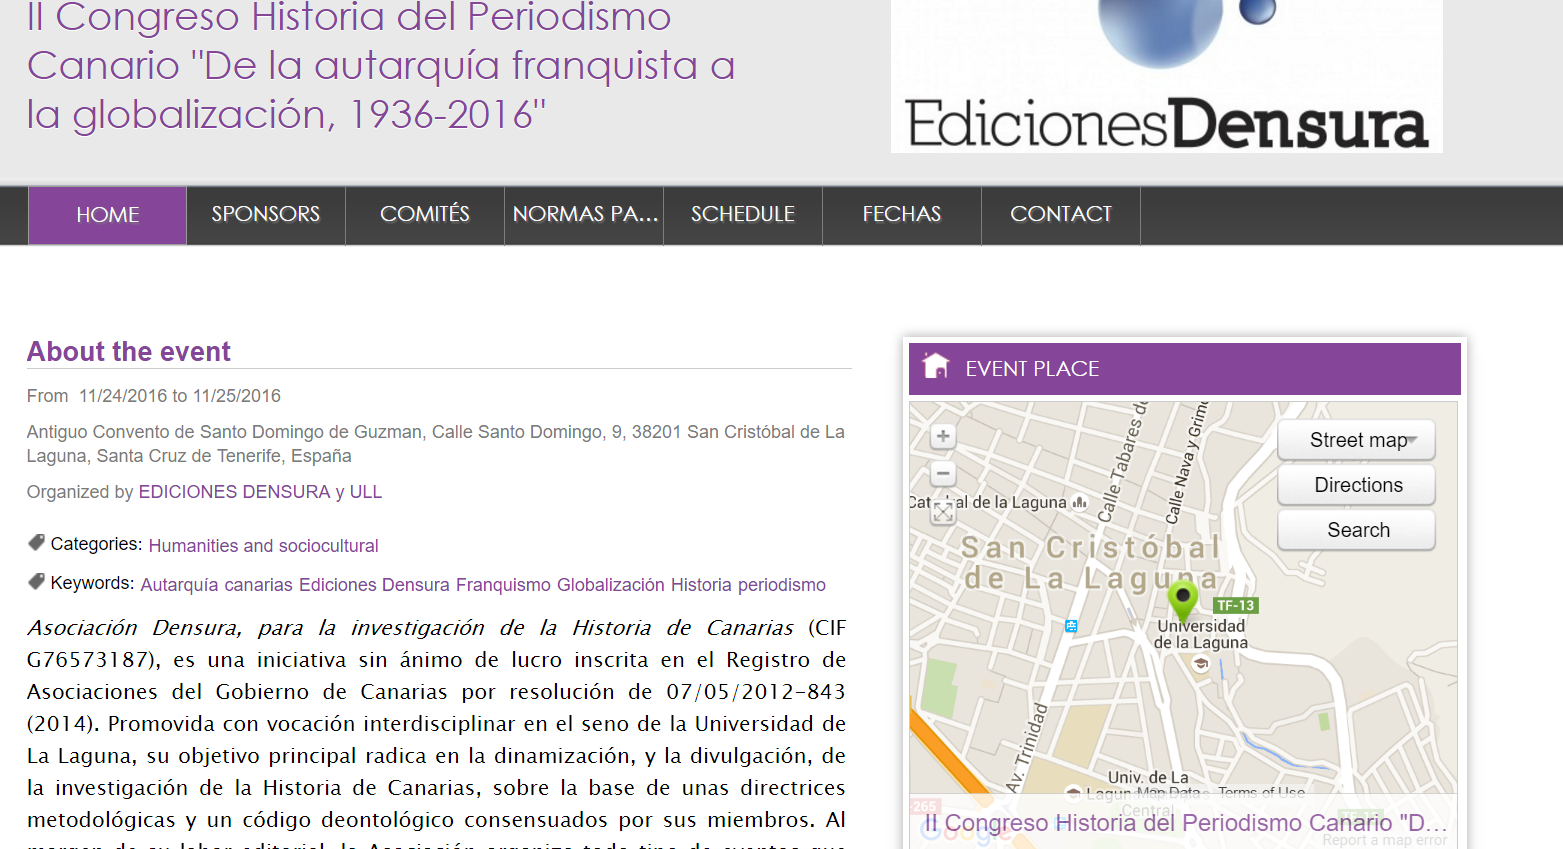
\includegraphics[width=\columnwidth]{eventsPage}
	\caption{La página web de eventos, donde podemos tener más información de un evento concreto.}
	\label{fig:eventsPage}
\end{figure}

\subsubsection{Dificultades}


A la hora de plantear este caso de uso no ha habido grandes dificultades, si bien la fuente de datos no ha sido la óptima, ya que lo ideal hubiese sido poder filtrar los eventos por localización en lugar de por categorías. Sin embargo, se ha conseguido el objetivo principal de mostrar diferentes eventos en función del beacon detectado.

\subsubsection{Ampliación}


Ampliar este caso de uso solo conllevaría asociar los nuevos identificadores de los beacons a nuevos identificadores de ficheros RSS. Es por ello que podemos afirmar que sería relativamente sencillo desplegar una red de beacons en diferentes puntos del campus universitario asociados a un RSS. En caso de utilizar otro medio al RSS, sólo habría que adaptar la obtención y la visualización del nuevo contenido, modificando la dirección y añadiendo un nuevo parseo.


\subsection{Control de asistencia}

\subsubsection{Objetivo}

Este caso de uso tiene como objetivo controlar la asistencia de los alumnos a las clases. En un principio se había descartado por las complicaciones que presentaba: 

\begin{itemize}
\item Era necesario tener un servidor en el que poder almacenar la información de las asistencias con la información del alumno.
\item Se necesitaba un modo de almacenar los datos del usuario para poder identificarle a la hora de registrar la asistencia.
\item El área de acción para registrar la asistencia podía ser variable, sin ser muy exacta. El rango podía salirse del aula o localización de la actividad.
\item Debía haber algún tipo de control para no registrar asistencias erróneas o fraudulentas.
\end{itemize}

Para solucionar estos problemas se ha optado por las siguientes soluciones: 

Como servidor se ha utilizado \textit{"`Couchbase Server"'}, una base de datos distribuida no-SQL, orientada a documentos y de código abierto. Por otro lado, se ha configurado en la aplicación móvil una base de datos \textit{"`Couchbase Lite"'} que sirve de paso intermedio e interactúa con \textit{"`Sync Gateway"'} para sincronizar los datos de la base de datos del dispositivo al servidor, y viceversa.


Para almacenar los datos del usuario se ha hecho uso de la API de preferencias de android, el cual almacena los datos en el dispositivo móvil en un espacio compartido para toda la aplicación. De esta manera, hemos almacenado datos como \textit{"`Nombre de Usuario"'}, \textit{"`Número Das"'} o \textit{"`DNI"'}, los cuales solo serán visibles para el usuario de la aplicación y servirán para dejar registradas las asistencias con estos datos. Al mismo tiempo, se almacena también la dirección MAC del dispositivo móvil para evitar replicaciones o falsos positivos.


En cuanto al área de acción a partir de la cual es posible guardar la asistencia, se ha optado por establecer un perímetro dentro del aula delimitado por las paredes del aula, menos cierto margen, de manera que el aula quede cubierta y los exteriores no se tengan en cuenta. 

\subsubsection{Despliegue}

En este caso, para poder realizar este proceso es necesario utilizar la trilateración \cite{URL::trilateracion} por lo que, es necesario desplegar al menos 3 beacons. Para las pruebas se ha utilizado el aula 2.1 del Edificio de Ingeniería Informática. Estos beacons no tienen que ser necesariamente por aula ya cada beacon cubre un área de 70 metros aproximadamente; teniendo en cuenta que las paredes crean interferencias en la señal, probablemente se podrían utilizar 3 beacons para cubrir dos aulas, pero habría que hacer un estudio de la localización y las interferencias para poder asegurarlo. 

\subsubsection{Funcionamiento}


En cuanto se accede al módulo de asistencia, la aplicación comienza a escanear las inmediaciones buscando beacons. Cuando detecta más de 3 beacons, la aplicación carga la imagen de dicha localización y comprueba que el alumno se encuentra dentro de la zona delimitada para registrar la asistencia.

\begin{figure}[H]
	\centering
	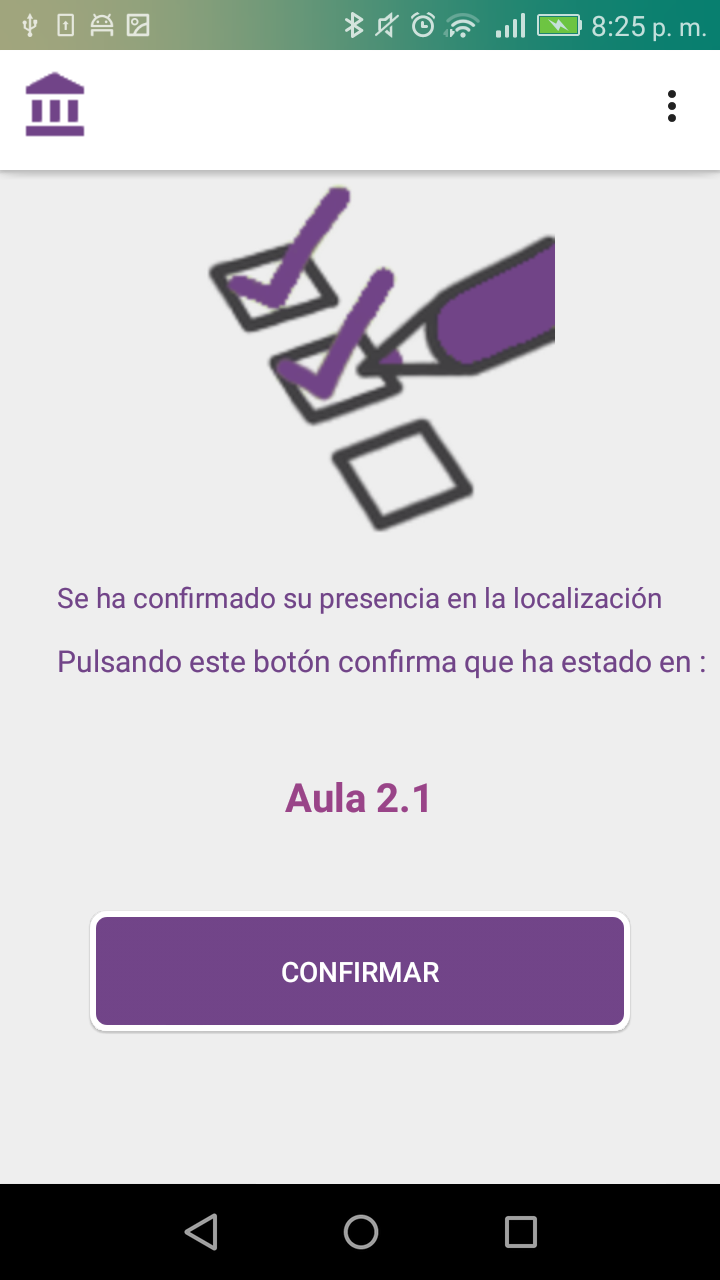
\includegraphics[width=120mm,height=170mm]{ConfirmarAsistencia}
	\caption{Pantalla de confirmación de asistencia en la localización.}
	\label{fig:confirmarAsistencia}
\end{figure}

Si no se encuentra en la zona delimitada, igualmente la aplicación muestra su ubicación en el mapa para que pueda corregir su posición. Una vez que acceda al área se muestra un mensaje de confirmación con el aula en la que se encuentra. En este momento se debe confirmar pulsando un botón de que deseas registrar la asistencia. Previamente el usuario ha debido introducir sus datos en la aplicación y ya deben estar guardados. Estos datos son los que utiliza la aplicación, junto con la dirección MAC del dispositivo desde el cual se manda la petición de registro. Otro control es almacenar una hora junto con los demás datos, a la hora de enviar la información al servidor, asegurándonos de que realmente el usuario ha estado en el aula a dicha hora.


Los datos que se almacenan en el servidor tienen la siguiente estructura, sin embargo esta estructura puede ser fácilmente modificada si se detecta que es necesario añadir más datos: 

\begin{figure}[H]
	\centering
	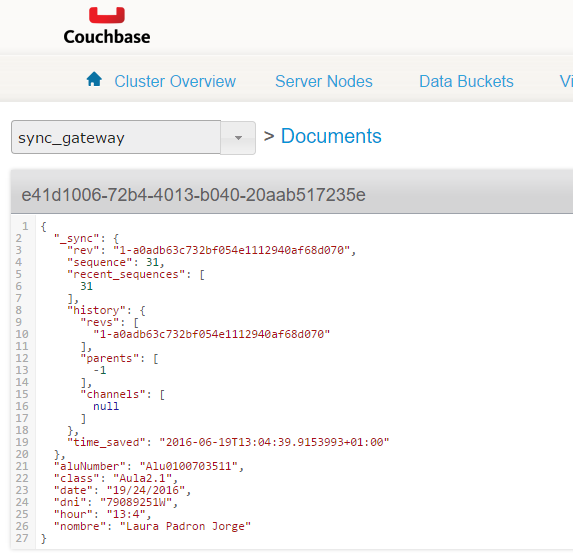
\includegraphics[width=\columnwidth]{couchDBstucture}
	\caption{La estructura de los datos del usuario en CouchBase Server.}
	\label{fig:couchDBstucture}
\end{figure}


\subsubsection{Dificultades}

En este caso las dificultades han sido de diversa índole, se ha tenido que configurar un servidor con el que no se había trabajado previamente, se ha tenido que trabajar con la API de preferencias de android, y había que idear un método que permitiese comprobar de manera fiable que el alumno se encontraba o había estado en la localización a la hora correcta. La configuración del servidor y Sync Gateway ha sido un poco tediosa, pero una vez configurada es muy fácil de utilizar.


\subsubsection{Ampliación}

Para ampliar este caso de uso se deberían incluir nuevos beacons, nuevas imagenes de las localizaciones y nuevas áreas de registro; sin embargo, el envío de datos sería practicamente el mismo. Si se decidiese cambiar en un futuro los datos a almacenar en el servidor, sería posible sin mucho esfuerzo.

\subsection{Guía a través del Campus de la Universidad}

\subsubsection{Objetivo}

Este caso de uso se centra en ofrecer una pequeña guía al usuario mostrándole su posición en un edificio y algo de información útil, en este caso hemos tomado de ejemplo el edificio de Matemáticas y Física ya que poseíamos los planos. 

En este caso se ha tomado como referencias algunas zonas del edificio y se han creado algunas indicaciones básicas para acompañar la posición en el mapa y los puntos de interés. Es necesario destacar que las pruebas se ha realizado utilizando 3 beacons, con lo cual sólo se ha cubierto una pequeña parte del edificio, sin embargo a modo de ejemplo muestra perfectamente las posibilidades de esta tecnología.

\subsubsection{Despliegue}

En este caso, también en necesario utilizar el algoritmo de trilateración, por lo que hemos tenido que desplegar 3 beacons en el lugar que queríamos visualizar, en el edificio de Física y Matemáticas en la primera planta, se han puesto en las esquinas de la zona principal, conserjería, cerca de los ascensores y en la entrada a los pasillos pricipales.

\subsubsection{Funcionamiento}


En cuanto se accede al módulo de guía, la aplicación comienza a escanear las inmediaciones buscando beacons. Cuando detecta más de 3 beacons, la aplicación carga la imagen de dicha la localización, en este caso el plano del edificio de Física y Matemáticas, una versión reducida para la parte en la que nos encontremos y comprueba que el alumno se encuentra dentro de algunas de las posibles zonas, en cuanto se entre en alguna se mostrará la información relacionada con esta posición. Ahora mismo las acciones de la zona se limitan a mostrar un pequeño texto con información generada teniendo en cuenta que el usuario necesite guiarse en las intalaciones, es decir, no se conoce las instalaciones.


Ya que este caso de uso podría ser útil para un rango más amplio de personas por su naturaleza de guía, se ha decidido ofrecer soporte en Inglés a la hora de mostrar las indicaciones.

\subsubsection{Dificultades}

Las dificultades de este caso de uso radican principalmente en situar al usuario en el edificio. Dentro de un edificio existen muchos factores que pueden distorsionar la calidad de la señal que emite un beacon (paredes, personas, etc.), y por tanto influir en su posición estimada en el mapa. A la hora de enfrentarnos a este problema hemos comprobado que la localización presenta un rango de error y que es necesario darle un margen de tiempo a la aplicación para calcular la posición del usuario. Para intentar paliar esta situación, las áreas en las que se intercambia información con el usuario aparecen pintadas en el mapa, de esta manera el usuario es capaz de saber con certeza que tiene un área de información e intentar corregir su posición si está interesado. 

\subsubsection{Ampliación}

Para ampliar este caso de uso se deberían incluir nuevos beacons, nuevas imagenes de las localizaciones (Exteriores o interiores) y nuevas áreas; Las áreas podrían ofrecer diferentes funcionalidades aparte de la información de la localización.


\subsection{Acceso al Parking}

\subsubsection{Objetivo}

El objetivo principal de este caso de uso es permitir a usuario acceder al parking utilizando la aplicación móvil. Actualmente el acceso al parking se formaliza utilizando tarjetas de acceso magnetizadas, el objetivo principal es poder sustituir este método por uno más sencillo y más sostenible a largo plazo. 

\subsubsection{Despliegue}

En este caso, también en necesario utilizar el algoritmo de trilateración, por lo que hemos tenido que desplegar 3 beacons en la entrada del parking, se ha utilizado el parking del edificio central, disponiendo los beacons en posiciones previamente seleccionadas como se muestra en la siguiente imagen.

\begin{figure}[H]
	\centering
	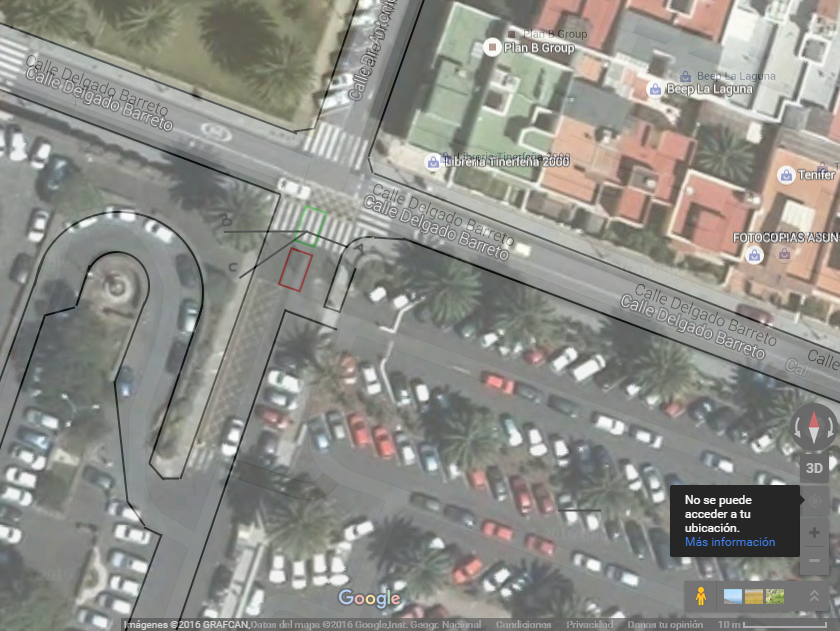
\includegraphics[width=140mm,height=120mm]{Parking}
	\label{fig:parking}
	\caption{Se puede apreciar la estructura del parking central, los puntos A, B y C señalan las posiciones de los beacons.}
\end{figure}

\subsubsection{Funcionamiento}


En cuanto se accede al módulo de parking, la aplicación muestra una lista con los diferentes parkings y el número de plazas de cada recinto. Esta lista se obtiene mediante una consulta a una API diseñada en colaboración con Alberto Morales, quién se ha encargado de montar el servicio para facilitar a la aplicación la información necesaria. De la lista de parkings, el usuario ha de seleccionar al que quiere acceder, identificando así la imagen y zonas a dibujar. Esta selección da paso a un escáner que comienza a detectar la posición del usuario y a situarlo en la imagen. Si el usuario se encuentra en una de las zonas designadas para entrar o salir del parking, se lanzará la acción, en este caso una petición de abertura contra el servidor. En este caso cada zona posee un identificador de barrera que es el que usa la petición para saber que barrera debe abrir. 


Por otro lado esta petición debe ir autentificada, para poder acceder, por lo que la aplicación ha negociado previamente un secreto con el servidor que la identifica y le permite realizar la acción de apertura utilizando un número identificativo basado en la MAC del dispositivo de pruebas.


\subsubsection{Dificultades}

En este caso de uso las dificultades han radicado en el hecho de comunicarse con el servidor para realizar las llamadas, la trilateración se ha realizado de la misma manera por lo que no ha habido grandes problemas. Además de estas dificultades, cabe añadir una adicional y es que la seguridad del parking depende del single log in de la ULL, por lo que ha habido que buscar la manera de abordar este tema. Sin embargo, Alberto se ha implicado en todo momento intentado resolver las necesidades de la aplicación de la manera más óptima, lo que ha sido una gran ayuda.

\subsubsection{Ampliación}

Para ampliar este caso de uso se deberían incluir nuevos beacons, 3 mínimo por cada recinto, nuevas imagenes de las localizaciones (Exteriores o interiores) y nuevas áreas; Las áreas serían vitales para definir las acciones de apertura de las barreas. Si las zonas acaban siendo muchas, sería recomendable crear una base de datos  para almacenar las localizaciones, las zonas y las imágenes a cargar.

\section{Despliegue}

El despliegue de estos dispositivos es variable como hemos podido comprobar con los distintos casos de uso. Sin embargo hay ciertas consideraciones que se cumplen en todos los casos, si lo que deseamos es un sistema que detecte entradas y salidas, independientemente de la posición exacta del usuario, simplemente necesitaremos un único beacon como regla general. 


Sin embargo, si deseamos conocer la localización más precisa del usuario necesitaremos recurir a un método como la Trilateración \cite{URL::trilateracion}. Serán necesarios mínimos 3 beacons, incrementando el número de beacons es posible aumentar la precisión con la que se percibe la posición del usuario. El algoritmo no es totalmente exacto, puesto que depende de las distancias calculadas a los beacons, sin embargo estas distancias pueden variar. Existen diversos factores que pueden influir en la calidad de la señal del Bluetooth y por tanto distorsionar estas distancias, entre otros factores podemos destacar principalmente:


\begin{itemize}
\item Físicos:  paredes, personas o elementos del entorno principalmente.
\item Intangibles: interferencias con otras ondas.
\item Configurables: la intensidad de la señal y por tanto su rango es configurable.
\end{itemize}


Todos estos factores han de ser tomados en cuenta a la hora de realizar el despligue de los beacons, otro factor a tener en cuenta es la altura, los dispositivos es recomendables levantarlos cierta altura del suelo, a la hora de probarlos se ha intentado, en la medida de lo posible, mantenerlos a un nivel elevado sobre la altura de las personas y siempre intentando mantener esta medida de altura para los diferentes beacons. En cuanto al despliegue de la aplicación, el código fuente se encontrará disponible para su descarga en el enlace \cite{URL::repositorioAplicacion}, bajo licencia Creative Commons Reconocimiento-NoComercial-CompartirIgual 4.0 Internacional \cite{URL::licencia}.
 
